\documentclass[submission,copyright,creativecommons]{eptcs}
%\providecommand{\event}{SOS 2007} % Name of the event you are submitting to
\usepackage{breakurl}             % Not needed if you use pdflatex only.

\usepackage{datetime}

\newdate{date}{04}{18}{2018}

\date{\displaydate{date}}

\title{Blockchain principles applied to transaction operations on the Real Estate Market}

\author{Andres Salgado

\institute{International Technological University\\ San Jose, California, \underline{USA}}
\email{salgadoandre533@students.itu.edu}
\and
Co Authors \qquad\qquad Jorge Valdeiglesias, Kartikeya Yellayi
\institute{International Technological University\\ San Jose, California, \underline{USA}}
\email{\quad valdeiglesjorge744@students.itu.edu \quad\qquad yellayishiva1284@students.itu.edu}
}

\def\titlerunning{Blockchain principles applied to transaction operations on the Real Estate Market}
\def\authorrunning{R.J. van Glabbeek, C. Author \& Y.S. Else}

\usepackage{graphicx} %package to manage images
\graphicspath{ {images/} }

\usepackage[rightcaption]{sidecap}

\usepackage{wrapfig}

\begin{document}
\maketitle
\displaydate{date}

\begin{abstract}
This is a sentence in the abstract.
This is another sentence in the abstract.
This is yet another sentence in the abstract.
This is the final sentence in the abstract.
\end{abstract}

\section{Introduction}

With the advent of ``blockchain'' technologies, as well as the necessity to establish a system where the trust of transactions could be offloaded to machines, we ventured into exploring how a system based on the Ethereum blockchain could accurately execute a series of smart contracts in order to validate a transaction between two entities.

%By means of the style-file option
%\href{http://creativecommons.org/about/license/}{creativecommons}
%authors equip their paper with a Creative Commons license that allows
%everyone to copy, distribute, display, and perform their copyrighted
%work and derivative works based upon it, but only if they give credit%the way you request. By invoking the additional style-file option {\tt
%noderivs} you let others copy, distribute, display, and perform only
%verbatim copies of your work, but not derivative works based upon
%it. Alternatively, the {\tt sharealike} option allows others to
%distribute derivative works only under a license identical to the
%license that governs your work. Finally, you can invoke the option
%{\tt noncommercial} that let others copy, distribute, display, and
%perform your work and derivative works based upon it for
%noncommercial purposes only.


\section{The blockchain and its influence on crypto-currencies}

It's close to 10 years after Bitcoin was introduced by Satoshi Nakamoto. The reason crypto-currencies currently exist is due to the underlying technology made available by the blockchain. Thomas Lowenthal from Ars Technica \cite{lowenthalBitcoinEncryptedPeertopeer2011} goes onto explaining the complexities of cryptographic currencies, the concept of mining and make-work, and goes onto comparing Bitcoin against the trusty greenback which also faced hurdles when it was first put into circulation.

The primary reason why cryptocurrencies are being adopted by a sizable portion of the population is due to the engineering concept behind the implementation of the blockchain to solve two basic problems inherit to digital currencies, the double-spending problem, and the prevention of counterfeiting\cite{noauthor_bitcoin}.
On cppcon 2016 David Schwarz\cite{cppconCppCon2016David} spoke about "Developing Blockchain Software".  On his talk he mentions key characteristics of "the blockchain". Section 2.1 goes onto describing such characteristics.   

\subsection{What is a blockchain and what is one good for?}
\begin{itemize}
\item Blockchains record state and history
\item State is modified by transactions
\item Everyone eventually agrees on the transactions
\item Can be used to transfer tokens
\end{itemize}

Based on this list, most of us would conclude that the blockchain is merely a database, but in actuality, the blockchain -according to Schwarz\cite{cppconCppCon2016David}- manages the double-spending problem.
\subsection{What the blockchain does for bitcoin}

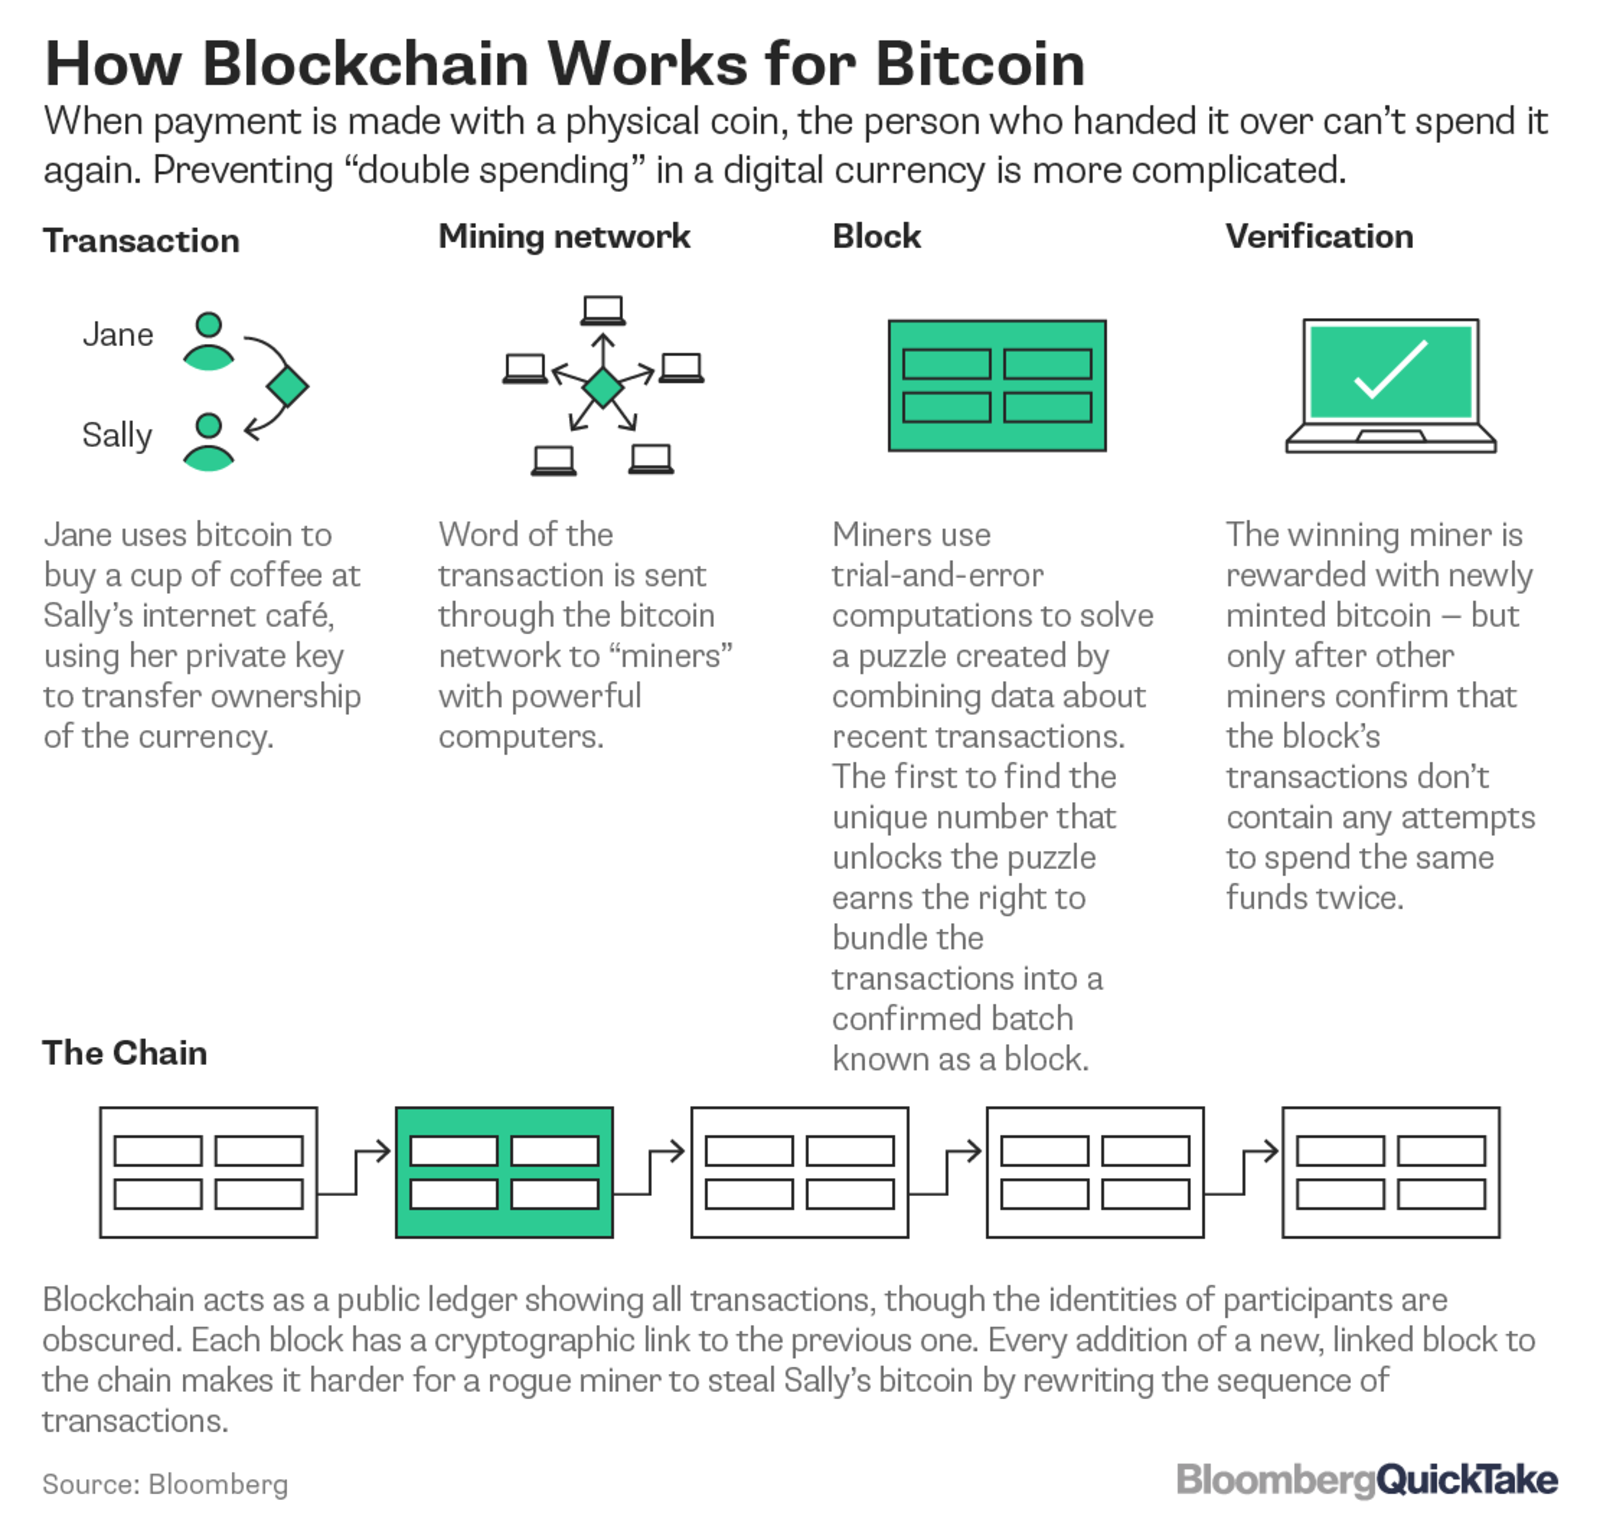
\includegraphics{bitcoin-blockchain-bloomberg}

Besides solving the issue of how to allow for a feasible digital currency, the blockchain has opened the door towards the development of new uses of the technology, that do not necessarily address the exchange of assets in a digital manner.


\section{Bibliography}

We request that you use
\href{http://www.cse.unsw.edu.au/~rvg/EPTCS/eptcs.bst}
{\tt $\backslash$bibliographystyle$\{$eptcs$\}$}. Compared to the original {\LaTeX}
{\tt $\backslash$biblio\-graphystyle$\{$plain$\}$},
it ignores the field {\tt month}, and uses the extra
bibtex fields {\tt eid}, {\tt doi}, {\tt ee} and {\tt url}.
The first is for electronic identifiers (typically the number $n$
indicating the $n^{\rm th}$ paper in an issue) of papers in electronic
journals that do not use page numbers. The other three are to refer,
with life links, to electronic incarnations of the paper.

Almost all publishers use digital object identifiers (DOIs) as a
persistent way to locate electronic publications. Prefixing the DOI of
any paper with {\tt http://dx.doi.org/} yields a URI that resolves to the
current location (URL) of the response page\footnote{Nowadays, papers
  that are published electronically tend
  to have a \emph{response page} that lists the title, authors and
  abstract of the paper, and links to the actual manifestations of
  the paper (e.g.\ as {\tt dvi}- or {\tt pdf}-file). Sometimes
  publishers charge money to access the paper itself, but the response
  page is always freely available.}
of that paper. When the location of the response page changes (for
instance through a merge of publishers), the DOI of the paper remains
the same and (through an update by the publisher) the corresponding
URI will then resolve to the new location. For that reason a reference
ought to contain the DOI of a paper, with a life link to corresponding
URI, rather than a direct reference or link to the current URL of
publisher's response page. This is the r\^ole of the bibtex field {\tt doi}.
DOIs of papers can often be found through
\url{http://www.crossref.org/guestquery};\footnote{For papers that will appear
  in EPTCS and use \href{http://www.cse.unsw.edu.au/~rvg/EPTCS/eptcs.bst}
  {\tt $\backslash$bibliographystyle$\{$eptcs$\}$} there is no need to
  find DOIs on this website, as EPTCS will look them up for you
  automatically upon submission of a first version of your paper;
  these DOIs can then be incorporated in the final version, together
  with the remaining DOIs that need to found at DBLP or publisher's webpages.}
the second method {\it Search on article title}, only using the {\bf
surname} of the first-listed author, works best.  
Other places to find DOIs are DBLP and the response pages for cited
papers (maintained by their publishers).
{\bf EPTCS requires the inclusion of a DOI in each cited paper, when available.}

Often an official publication is only available against payment, but
as a courtesy to readers that do not wish to pay, the authors also
make the paper available free of charge at a repository such as
\url{arXiv.org}. In such a case it is recommended to also refer and
link to the URL of the response page of the paper in such a
repository.  This can be done using the bibtex fields {\tt ee} or {\tt
url}, which are treated as synonyms.  These fields should not be used
to duplicate information that is already provided through the DOI of
the paper.
You can find archival-quality URL's for most recently published papers
in DBLP---they are in the bibtex-field {\tt ee}. In fact, it is often
useful to check your references against DBLP records anyway, or just find
them there in the first place.

When using {\LaTeX} rather than {\tt pdflatex} to typeset your paper, by
default no linebreaking within long URLs is allowed. This leads often
to very ugly output, that moreover is different from the output
generated when using {\tt pdflatex}. This problem is repaired when
invoking \href{http://www.cse.unsw.edu.au/~rvg/EPTCS/breakurl.sty}
{\tt $\backslash$usepackage$\{$breakurl$\}$}: it allows linebreaking
within links and yield the same output as obtained by default with
{\tt pdflatex}. 
When invoking {\tt pdflatex}, the package {\tt breakurl} is ignored.

The optional arguments of {\tt $\backslash$documentclass$\{$eptcs$\}$} are
\begin{itemize}
\item at most one of
{\tt adraft},
{\tt submission} or
{\tt preliminary},
\item at most one of {\tt publicdomain} or {\tt copyright},
\item and optionally {\tt creativecommons},
  \begin{itemize}
  \item possibly augmented with
    \begin{itemize}
    \item {\tt noderivs}
    \item or {\tt sharealike},
    \end{itemize}
  \item and possibly augmented with {\tt noncommercial}.
  \end{itemize}
\end{itemize}


\bibliographystyle{unsrt}
\bibliography{biblio}
\end{document}
